
\subsection{Lagrange Multipliers and Optimization}
In Calculus I, you saw methods for constrained optimization. In particular, given a function with $n$ inputs and $n-1$ constraints, you could generally use the constraints to rewrite the function as a single input function, then simply find a maximum value. Using multivariate techniques, we can generalize these ideas a little further.

\begin{claim}{Gradient is Perpendicular to Level Curves}
Let $f(x,y)$ be a function, and $\nabla f(x,y)$ be the gradient of that function. Then for any $(x_0,y_0)$ in the domain of $f$, $\nabla f(x_0,y_0)$ is normal to (read perpendicular to) the level curve $f(x_0,y_0)=f(x,y)$ at $(x_0, y_0)$.
\end{claim}

That's an interesting claim. To justify it, we can both look at an example, and think about what the gradient represents. Firstly, let's think about the gradient. The gradient of $f$ is a vector function with a vector input. It takes some $(x,y)$ as input and returns a 2-dimensional vector as output. So a great way to visualize the gradient is as a slope field. This basically takes each $(x,y)$ input and draws a vector with the direction of $\nabla f$ at each point.

\vspace{1em}
\begin{center}
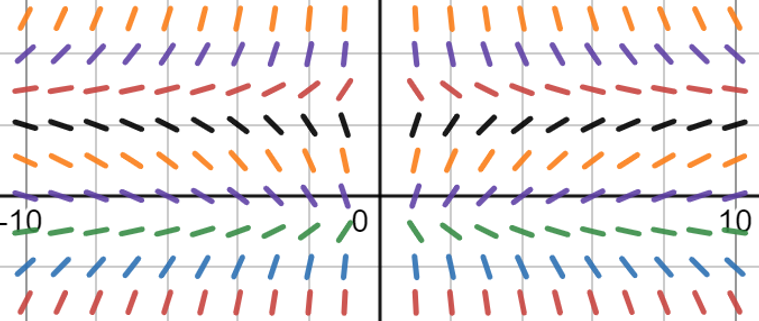
\includegraphics[scale=0.5]{Figures/slopefieldex1}
\\ Slope Field for $\nabla f$, where $f=10-x^2+y^3-3y^2-6y$.
\end{center}
\vspace{1em}

So what information does this actually tell us? Well, the gradient points us in the direction of maximal ascent of a surface. So if you're standing at $(x_0,y_0)$ on the surface of $f$, then the gradient tells you what direction you should turn to ascend as quickly as possible.

Another way to think of that is, if you're standing at $(x_0,y_0)$ on the surface of $f$, then consider the plane tangent to $f$ at $(x_0,y_0)$. This plane should have some ``flat" line you can walk along, some line parallel to the $xy$-plane. The gradient will be perpendicular to that line.

Let's look at an example!

\begin{example}{Gradient and Level Curves}
Let's keep using the function $f(x,y)=10-x^2+y^3-3y^2-6y$. We will consider the point at $x=1$, $y=1$. Then $f(x,y)=10-1^2+1^3-3(1)^2-6(1)=1$. Additionally, $$\nabla f(1,1)=\bmat{-2(1)\\3(1^2)-6(1)-6}=\bmat{-2\\-9}.$$
We can see the situation in the graph below. The black curve is the level curve $1=f(x,y)$. The blue vector is the gradient padded out with a $z$-coordinate of $0$, moved over to begin at $(1,1,1)$ for clarity. The red line is the line tangent to the normal curve. The purple plane is the tangent plane (not shown in the image below for clarity).
\vspace{1em}
\begin{center}
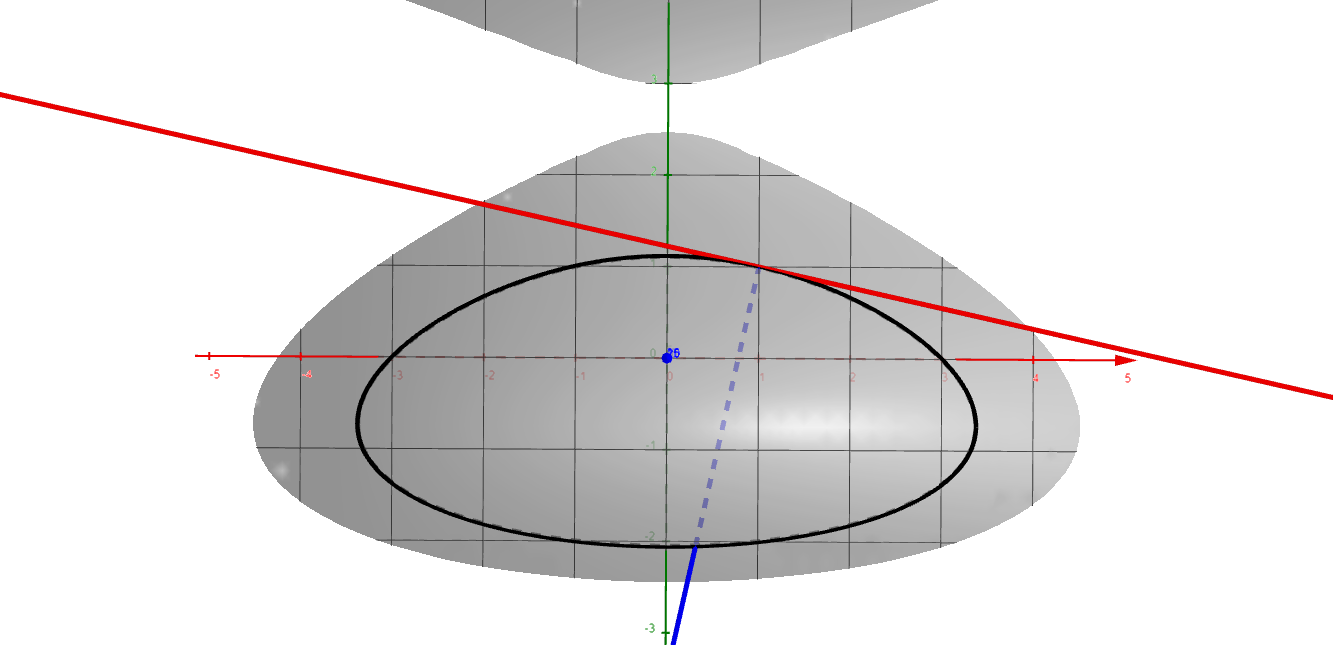
\includegraphics[scale=0.25]{Figures/normaltolevelex}\\
\href{https://www.geogebra.org/3d/w3hdn8w7}{Click Here for an interactable Geogebra Link.}
\end{center}
\vspace{1em}

If you go to the geogebra link, you can vary the values of $h$ and $k$ to explore this situation at an any given arbitrary $x=h$ and $y=k$. You should find that the gradient vector is always normal to the given level curve.

\vspace{1em}

But why is this the case? Let's try to get some intuition. Imagine you're standing at the point $A=(h,k,f(h,k))$ on this surface, and you want to climb to a higher altitude. The level curve at $A$ denotes the altitude that you are at, while the second level curve denotes the part of the surface that is at the higher altitude that you want to climb to.
\vspace{1em}
\begin{center}
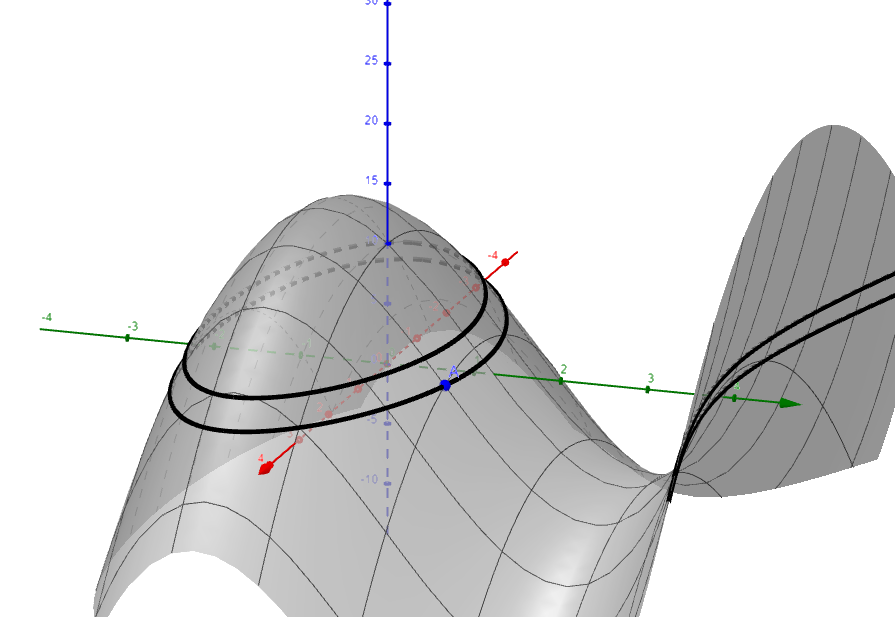
\includegraphics[scale=0.4]{Figures/gradperp1}\\
Point A and Level Curves.
\end{center}
\vspace{1em}
What direction should you head in to ascend as quickly as possible? Well, the direction to the closest point along the next level curve is perpendicular from your current level curve. 

\vspace{1em}

Let's consider the plane tangent to $f(x,y)$ at $A$. We learned in section 4.2 that the tangent plane should be parallel to the vectors $$\vcf_x=\bmat{1\\0\\f_x(h,k)}\text{ and } \vcf_y=\bmat{0\\1\\f_y(h,k)}.$$ We can calculate the cross product of those two vectors $$\vcf_y\times\vcf_x=\bmat{f_x(h,k)\\f_y(h,k)\\-1},$$ which is exactly the vector that is normal to the tangent plane. Since the line that is tangent to our level curve at $A$ is contained inside plane tangent to $f$ at $A$, this normal vector must be perpendicular to that line tangent to the level curve (the red line from the figure earlier in this example). Then notice that if you truncate off the $z$-coordinate from our normal vector, $$ \bmat{f_x(h,k)\\f_y(h,k)\\-1}\to \bmat{f_x(h,k)\\f_y(h,k)}=\nabla f(h,k).$$ This is exactly the gradient of $f$ evaluated at $(h,k)$. Therefore, the gradient gives us the direction that is perpendicular to our level curve, which points us in the direction of steepest ascent.
\vspace{1em}
\end{example}

Why does this matter? Well, it's key to a method of optimization called \textbf{Lagrange multipliers}. Essentially, given some surface $f(x,y)$ and a constraint curve $g(x,y)=c$, any maximum or minimum of the intersection of the surface and constraint will be found at a point where the gradient of the surface and the gradient of the constraint point in the same direction. We don't care about the magnitude of the gradients, so that introduces the nominal multiplier. More specifically:

\begin{theorem}{Lagrange Multipliers}
Let $z=f(x_1,\ldots, x_n)$ be a function and $c=g(x_1,\ldots,x_n)$ be a constraint curve. Then any max or min of $f$ along $g(x,y)=c$ will be found at a point satisfying the equation $$\nabla f=\lambda \nabla g $$ where $\lambda$ is some constant.
\end{theorem}

In particular, note that $\nabla f=\lambda \nabla g$ yields exactly $n$ equations with $n+1$ unknowns. So if you include the constraint itself, you have a system of equations with $n+1$ equations and $n+1$ unknowns, so it is theoretically possible to solve for all of your unknown values. In practice, these systems are often non-linear in multiple variables and extremely difficult to solve by hand, but can be solved by computers.

\begin{example}{A Calculus I Problem made Harder.}
Suppose we want to build a square bottomed box with a double thickness base and we have exactly $8$ square meters of materials. How should we build the box to maximize the volume contained in the box? First, let's start by identifying an objective function and a constraint curve. Here, our objective is volume. Since the base of the box is square, we can write our volume function as $$f(x,y)=x^2y.$$
Then our constraints should be the surface area of the box. We need a double thickness base, so we will have four sides of area $xy$, the top will be area $x^2$ and the bottom will need two slabs of area $x^2$. Since we have exactly 8 square meters of material, this leaves the constraint $$8=4xy+3x^2. $$ If you follow this \href{https://www.geogebra.org/3d/azxkj796}{Geogebra Link}, you'll be able to see a graph of the surface $f(x,y)$ and the constraint, $8=4xy+3x^2$. The intersection of these two surfaces is the path that we are trying to find the highest point along. To do that, we'll use our Lagrange multiplier to try to identify where our gradients are parallel. Note that in this case, $g(x,y)=4xy+3x^2$. So then our gradients in question are $$\nabla f(x,y)=\bmat{2xy\\x^2}, \text{ and }\nabla g(x,y)=\bmat{4y+6x\\4x} $$
and our Lagrange multiplier condition is $$\bmat{2xy\\x^2}=\lambda\bmat{4y+6x\\4x}. $$
This yields the following system of 3 unknowns and 3 equations:
\begin{align*}
2xy=&\lambda(4y+6x)\\
x^2=&4\lambda x\\
8=&4xy+3x^2.
\end{align*}
This system of equations yields that $x=\frac{2\sqrt{2}}{3}$ and $y=\sqrt{2}$. It also finds that $\lambda=\frac{\sqrt{2}}{6}$, which isn't necessary for our solution but a useful intermediary step. 
\end{example}

\begin{exercise}{Something Geometric}
Consider the surface $$f(x,y)=5+2x-y$$ and the constraint curve $$1=x^2+\frac{y^2}{4}.$$ Find the maximum and minimum points of the surface along the constraint curve. You can see this surface and constraint at this \href{https://www.geogebra.org/3d/dxtzfpca}{Geogebra link}.
\end{exercise}

\begin{exercise}{Revisiting Point to Plane}
While earlier in the semester we solved the question of point to plane using geometry and projections, we can also consider the idea of finding the distance between a point and a plane as a constrained optimization problem. In this case, the function we are seeking to minimize is the distance between an arbitrary point and the point in question, and the constraint is the equation of the plane itself. Let $P=(1,3,2)$ and consider the plane $-x+y-2z=3$. 
\vspace{1em}
\begin{itemize}
\item What is the function that gives the distance, $d$, between $P$ and an arbitrary point, $(x,y,z)$? 
\vspace{1em}
\item Note that if we just use the distance formula blindly, while we get a technically solvable problem, it's a very \textit{gross} solvable problem. However, there's a nice trick here. Explain why minimizing the \textit{square} of the distance is the same as minimizing the distance! 
\vspace{1em}
\item Now using $f(x,y,z)=d^2$ and the constraint $-x+y-2z=3$, use Lagrange multipliers to find the minimum distance between the point and plane. 
\vspace{1em}
\item Verify that your distance is correct by using the projection method we studied earlier in the semester!
\end{itemize}
\end{exercise}

\begin{exercise}{Something Economic}
The Cobb-Douglas production model seeks to define production as a function of labor and capital. Call $x$ the amount of labor and $y$ the amount of capital invested into a project. Then the total cost of the project is $$c=ax+by.$$ The Cobb Douglas (with slight simplification and some assumptions) model claims that $P(x,y)$, the amount of production as a factor of $x$ amount of labor and $y$ amount of capital will be of the form $$P(x,y)=x^\alpha y^{1-\alpha} $$ for some real $\alpha$. Use Lagrange multipliers to calculate how much labor and capital should be applied in order to maximize production. Your answer should be stated in terms of $a,b,c$ and $\alpha$.
\end{exercise}